% -*- Mode:TeX -*-

%% IMPORTANT: The official thesis specifications are available at:
%%            http://libraries.mit.edu/archives/thesis-specs/
%%
%%            Please verify your thesis' formatting and copyright
%%            assignment before submission.  If you notice any
%%            discrepancies between these templates and the 
%%            MIT Libraries' specs, please let us know
%%            by e-mailing thesis@mit.edu

%% The documentclass options along with the pagestyle can be used to generate
%% a technical report, a draft copy, or a regular thesis.  You may need to
%% re-specify the pagestyle after you \include  cover.tex.  For more
%% information, see the first few lines of mitthesis.cls. 

%\documentclass[12pt,vi,twoside]{mitthesis}
%%
%%  If you want your thesis copyright to you instead of MIT, use the
%%  ``vi'' option, as above.
%%
%\documentclass[12pt,twoside,leftblank]{mitthesis}
%%
%% If you want blank pages before new chapters to be labelled ``This
%% Page Intentionally Left Blank'', use the ``leftblank'' option, as
%% above. 

\documentclass[12pt,twoside]{mitthesis}
\usepackage{lgrind}
\usepackage{graphicx}
\pagestyle{plain}

%% This bit allows you to either specify only the files which you wish to
%% process, or `all' to process all files which you \include.
%% Krishna Sethuraman (1990).

%\typein [\files]{Enter file names to process, (chap1,chap2 ...), or `all' to
%process all files:}
%\def\all{all}
%\ifx\files\all \typeout{Including all files.} \else \typeout{Including only \files.} \includeonly{\files} \fi

\begin{document}

%% -*-latex-*-
% 
% For questions, comments, concerns or complaints:
% thesis@mit.edu
% 
%
% $Log: cover.tex,v $
% Revision 1.8  2008/05/13 15:02:15  jdreed
% Degree month is June, not May.  Added note about prevdegrees.
% Arthur Smith's title updated
%
% Revision 1.7  2001/02/08 18:53:16  boojum
% changed some \newpages to \cleardoublepages
%
% Revision 1.6  1999/10/21 14:49:31  boojum
% changed comment referring to documentstyle
%
% Revision 1.5  1999/10/21 14:39:04  boojum
% *** empty log message ***
%
% Revision 1.4  1997/04/18  17:54:10  othomas
% added page numbers on abstract and cover, and made 1 abstract
% page the default rather than 2.  (anne hunter tells me this
% is the new institute standard.)
%
% Revision 1.4  1997/04/18  17:54:10  othomas
% added page numbers on abstract and cover, and made 1 abstract
% page the default rather than 2.  (anne hunter tells me this
% is the new institute standard.)
%
% Revision 1.3  93/05/17  17:06:29  starflt
% Added acknowledgements section (suggested by tompalka)
% 
% Revision 1.2  92/04/22  13:13:13  epeisach
% Fixes for 1991 course 6 requirements
% Phrase "and to grant others the right to do so" has been added to 
% permission clause
% Second copy of abstract is not counted as separate pages so numbering works
% out
% 
% Revision 1.1  92/04/22  13:08:20  epeisach

% NOTE:
% These templates make an effort to conform to the MIT Thesis specifications,
% however the specifications can change.  We recommend that you verify the
% layout of your title page with your thesis advisor and/or the MIT 
% Libraries before printing your final copy.
\title{An Optimizing Compiler for Low-Level Floating Point Operations}

\author{Lucien William Van Elsen}
% If you wish to list your previous degrees on the cover page, use the 
% previous degrees command:
%       \prevdegrees{A.A., Harvard University (1985)}
% You can use the \\ command to list multiple previous degrees
%       \prevdegrees{B.S., University of California (1978) \\
%                    S.M., Massachusetts Institute of Technology (1981)}
\department{Department of Electrical Engineering and Computer Science}

% If the thesis is for two degrees simultaneously, list them both
% separated by \and like this:
% \degree{Doctor of Philosophy \and Master of Science}
\degree{Bachelor of Science in Computer Science and Engineering}

% As of the 2007-08 academic year, valid degree months are September, 
% February, or June.  The default is June.
\degreemonth{June}
\degreeyear{1990}
\thesisdate{May 18, 1990}

%% By default, the thesis will be copyrighted to MIT.  If you need to copyright
%% the thesis to yourself, just specify the `vi' documentclass option.  If for
%% some reason you want to exactly specify the copyright notice text, you can
%% use the \copyrightnoticetext command.  
%\copyrightnoticetext{\copyright IBM, 1990.  Do not open till Xmas.}

% If there is more than one supervisor, use the \supervisor command
% once for each.
\supervisor{William J. Dally}{Associate Professor}

% This is the department committee chairman, not the thesis committee
% chairman.  You should replace this with your Department's Committee
% Chairman.
\chairman{Arthur C. Smith}{Chairman, Department Committee on Graduate Theses}

% Make the titlepage based on the above information.  If you need
% something special and can't use the standard form, you can specify
% the exact text of the titlepage yourself.  Put it in a titlepage
% environment and leave blank lines where you want vertical space.
% The spaces will be adjusted to fill the entire page.  The dotted
% lines for the signatures are made with the \signature command.
\maketitle

% The abstractpage environment sets up everything on the page except
% the text itself.  The title and other header material are put at the
% top of the page, and the supervisors are listed at the bottom.  A
% new page is begun both before and after.  Of course, an abstract may
% be more than one page itself.  If you need more control over the
% format of the page, you can use the abstract environment, which puts
% the word "Abstract" at the beginning and single spaces its text.

%% You can either \input (*not* \include) your abstract file, or you can put
%% the text of the abstract directly between the \begin{abstractpage} and
%% \end{abstractpage} commands.

% First copy: start a new page, and save the page number.
\cleardoublepage
% Uncomment the next line if you do NOT want a page number on your
% abstract and acknowledgments pages.
% \pagestyle{empty}
\setcounter{savepage}{\thepage}
\begin{abstractpage}
% $Log: abstract.tex,v $
% Revision 1.1  93/05/14  14:56:25  starflt
% Initial revision
% 
% Revision 1.1  90/05/04  10:41:01  lwvanels
% Initial revision
% 
%
%% The text of your abstract and nothing else (other than comments) goes here.
%% It will be single-spaced and the rest of the text that is supposed to go on
%% the abstract page will be generated by the abstractpage environment.  This
%% file should be \input (not \include 'd) from cover.tex.
In this thesis, I designed and implemented a compiler which performs
optimizations that reduce the number of low-level floating point operations
necessary for a specific task; this involves the optimization of chains of
floating point operations as well as the implementation of a ``fixed'' point
data type that allows some floating point operations to simulated with integer
arithmetic.  The source language of the compiler is a subset of C, and the
destination language is assembly language for a micro-floating point CPU.  An
instruction-level simulator of the CPU was written to allow testing of the
code.  A series of test pieces of codes was compiled, both with and without
optimization, to determine how effective these optimizations were.

\end{abstractpage}

% Additional copy: start a new page, and reset the page number.  This way,
% the second copy of the abstract is not counted as separate pages.
% Uncomment the next 6 lines if you need two copies of the abstract
% page.
% \setcounter{page}{\thesavepage}
% \begin{abstractpage}
% % $Log: abstract.tex,v $
% Revision 1.1  93/05/14  14:56:25  starflt
% Initial revision
% 
% Revision 1.1  90/05/04  10:41:01  lwvanels
% Initial revision
% 
%
%% The text of your abstract and nothing else (other than comments) goes here.
%% It will be single-spaced and the rest of the text that is supposed to go on
%% the abstract page will be generated by the abstractpage environment.  This
%% file should be \input (not \include 'd) from cover.tex.
In this thesis, I designed and implemented a compiler which performs
optimizations that reduce the number of low-level floating point operations
necessary for a specific task; this involves the optimization of chains of
floating point operations as well as the implementation of a ``fixed'' point
data type that allows some floating point operations to simulated with integer
arithmetic.  The source language of the compiler is a subset of C, and the
destination language is assembly language for a micro-floating point CPU.  An
instruction-level simulator of the CPU was written to allow testing of the
code.  A series of test pieces of codes was compiled, both with and without
optimization, to determine how effective these optimizations were.

% \end{abstractpage}

\cleardoublepage

\section*{Acknowledgments}

This is the acknowledgements section.  You should replace this with your
own acknowledgements.

%%%%%%%%%%%%%%%%%%%%%%%%%%%%%%%%%%%%%%%%%%%%%%%%%%%%%%%%%%%%%%%%%%%%%%
% -*-latex-*-

% % -*- Mode:TeX -*-
%
% Some departments (e.g. Chemistry) require an additional cover page
% with signatures of the thesis committee.  Please check with your
% thesis advisor or other appropriate person to determine if such a 
% page is required for your thesis.  
%
% If you choose not to use the "titlepage" environment, a \newpage
% commands, and several \vspace{\fill} commands may be necessary to
% achieve the required spacing.  The \signature command is defined in
% the "mitthesis" class
%
% The following sample appears courtesy of Ben Kaduk <kaduk@mit.edu> and
% was used in his June 2012 doctoral thesis in Chemistry. 

\begin{titlepage}
\begin{large}
This doctoral thesis has been examined by a Committee of the Department
of Chemistry as follows:

\signature{Professor Jianshu Cao}{Chairman, Thesis Committee \\
   Professor of Chemistry}

\signature{Professor Troy Van Voorhis}{Thesis Supervisor \\
   Associate Professor of Chemistry}

\signature{Professor Robert W. Field}{Member, Thesis Committee \\
   Haslam and Dewey Professor of Chemistry}
\end{large}
\end{titlepage}


\pagestyle{plain}

  % -*- Mode:TeX -*-
%% This file simply contains the commands that actually generate the table of
%% contents and lists of figures and tables.  You can omit any or all of
%% these files by simply taking out the appropriate command.  For more
%% information on these files, see appendix C.3.3 of the LaTeX manual. 
\tableofcontents
\newpage
\listoffigures
\newpage
\listoftables


%\include{chap1}
\chapter{Introduction}


The computational complexity of machine learning algorithms has become a limiting factor for problems that require processing large volumes of data and where the response time is crucial. An example of this is financial volatility time series forecast. 

Currently, it is known that volatility is a process where many factors influence its behaviour. However, many models of volatility made forecasts based only on price returns. Examples are the ARFIMA, GARCH and stochastic volatility models. Machines learning methods have allowed a greater number of explanatory variables to be included, although in many cases, these increase calculation time. 

Algorithms that process large amounts of data in a short time and are able to detect changes in the financial market are required to achieve fast and accurate responses. Online learning algorithms have been developed to solve large-scale problems since they process an instance at a time, updating the model at each step incrementally. This is opposed to the batch algorithms where a phase of training that uses a large collection of historical data is first required and the resulting model is later used to predict. 
This thesis proposal is to design and develop an online learning algorithm that meets or improves the performance of current volatility algorithms and ensures rapid responses to large-scale problems. Model comparisons will be made by the SPA (superior predictive ability) test proposed by Hansen and
Lunde~\cite{hansen+lunde2006}  that allows comparing of forecast models giving a relative measure of model performance with respect to one or more models.

%Keywords: Volatility, Machine learning, Online learning, large-scale learning

\section{The problem}

In financial markets, volatility is one of the key elements to model the stochastic dynamic behaviour of financial assets. This is mainly because volatility gives a measure of uncertainty about future returns and it is often viewed as an indicator of the vulnerability of financial markets. It is also important as an input parameter in problems like derivative pricing, hedging and portfolio management. For example, in option pricing we need to known first the volatility of the underlying asset before pricing an option. 

Besides, volatility provides important information for studying asset returns because the latter are largely uncorrelated and nonlinearly dependent. However, it has been found that volatility exhibits significant autocorrelation and predictable patterns~\cite{poon+granger2003} and  many models have been proposed to forecast its behaviour (see section ~\ref{sec:stylizedfacts}).

The volatility of the data is due to a large number of factors affecting the market, with some of them directly measurable such as historical prices, trends, supply and demand. However, others such as monetary policies and news are not directly measurable and are included in other models out of the scope of this thesis. Figure~\ref{fig:VolFactorNews} shows the VIX index, the daily US implied stock market volatility, commonly known as the "financial fear factor" which is clearly affected by historical events.


\begin{figure}[h]
 \centering
 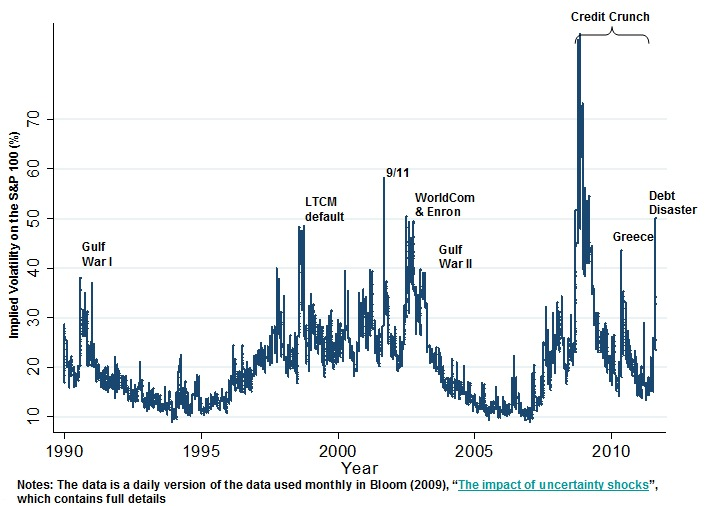
\includegraphics[width=0.7\textwidth]{img/vol-factor-thenews.jpg}
 % vol-factor-thenews.jpg: 710x506 pixel, 72dpi, 25.05x17.85 cm, bb=0 0 710 506
 \caption{The news as volatility factor}
 \label{fig:VolFactorNews}
\end{figure}


Volatility models have been extensively studied~\cite{gatheral2006,poon+granger2003,knight2002} and some of  them include machine learning methods~\cite{hamidetal2004,donaldsonetal1997,shiyietal2008,shiyietal2010,gavrishchaka2006,vasilios2012}.  
The stochastic behaviour of volatility and the large number of factors affecting it result in models with a large number of parameters and slow response time due to the computationally expensive routines. These expensive calculations could be avoided using online learning algorithms, which allow response time reduction and are therefore suitable for high frequency trading applications. 

In this thesis, a model will be proposed based on online learning algorithms to forecast volatility in high frequency financial time series.
The main problems to be deal with in this thesis are:

\begin{itemize}
   \item Although volatility is often predictable~\cite{poon+granger2003}, there are non-linear features~\cite{gatheral2006} to be considered in this proposal.
    \item The number of factors affecting volatility has been studied~\cite{srinivasan2009} and some other unknown factors affect volatility and they should also be included.
    \item The response time needs to be very fast and in order to ensure this, the proposed model will be presented as an online machine learning algorithm. 
\end{itemize}



\section{Volatility definition}

\begin{itemize}

\item Is the size of the price movement.

\item Variance is a measure of distribution of returns and is not neccesarily bound by any time period.
Volatility is a measure of the standard deviation (square root of the variance) over a certain time interval. In finance, variance and volatility both gives you a sense of an asset's risk. Variance gives you a sense of the risk in the asset over its lifetime, while volatility gives you a sense of the movement of the asset in eg. the past month or the past year.


\item The main underlying difference is in their definition. Variance has a fixed mathematical definition, however volatility does not as such. Volatility is said to be the measure of fluctuations of a process.

Volatility is a subjective term, whereas variance is an objective term i.e. given the data you can definitely find the variance, while you can't find volatility just having the data. Volatility is associated with the process, and not with the data.

In order to know the volatility you need to have an idea of the process i.e you need to have an observation of the dispersion of the process. All the different processes will have different methods to compute volatilities based on the underlying assumptions of the process.
\end{itemize}



\subsubsection{Types of volatility}

The volatility of a stock is not directly observable~\cite{tsay2005,engle1993}. For example, daily volatility is not directly observable from only daily returns because there is only one observation in a trading day.  If intraday data is available, then volatility could be estimated. However, intraday returns are not the only explanatory variables for volatility and several estimators have been proposed. These estimators are observable variables that are related to the latent variable of interest called volatility proxies~\cite{devilderetal2007}. Examples of volatility proxies are the following: 


\begin{description}%[leftmargin=0.4cm]\itemsep4pt
\item[realized volatility:] is also known as historic volatility and
it is the actual variance in the price of a stock over time.
Realized volatility is measured in terms of the standard deviation
using the historical stock prices. It is commonly calculated based on
intraday price returns:

\begin{equation}
\label{eq:retintra}
r_{t,n}=100(\ln(p_{t,n}) - \ln(p_{t,n-1}))
\end{equation}

\noindent where $p_{t,n}$ is the price observed at day $t=1,\dots,T$ and
intraday sample $n=2,\dots,N$. Realized volatility is defined as:

\begin{equation}
\label{eq:rv}
    \hat{\sigma}(t) = \sum_{n=1}^N r_{t,n}^2 \, , 
\end{equation}

\noindent where $N$ is the number of intraday samples and $T$ is the
number of days. 

In order to include overnight returns, Hansen and
Lunde~\cite{hansen+lunde2005} introduced a scaling version of
realized volatility using the following definitions:

\begin{eqnarray}
r_{t}&=&100(\ln(p_{t,N}) - \ln(p_{t-1,N})) \label{eq: ret 1} \\
\bar{\rho}(t) &=& \sum_{t=1}^T r_{t}^2  \label{eq: ret 2} \, .
\end{eqnarray}

\noindent where equation~(\ref{eq: ret 1}) represents overnight 
returns and the volatility as 
equation~(\ref{eq: ret 2}), where $p_{t,N}$ is the last intraday 
sample at day $t$. The scaled realized volatility $\rho(t)$ is 
defined as:

\begin{eqnarray}
\label{eq:srv}
\rho(t) = \gamma \hat{\rho}(t) \, , \qquad & \qquad \gamma = \displaystyle \frac{\bar{\rho}(t)}{\displaystyle\sum_{t=1}^T \hat{\rho}(t)}
\end{eqnarray}


Realized volatility has also been defined as the absolute value return or as the mean of the sum of intraday squared returns at short intervals of time. The majority of research carried out in the literature obtain the daily volatility as the daily squared returns as is shown in equation~(\ref{eq: ret 2}).  However, it has been proven that this measurement noise is too high for observing the true volatility process~\cite{andersen+bollerslev1998}. Hansen and Lunde~\cite{hansen+lunde2006} stated that the use of a noisy proxy could result in an inferior model being chosen as the best one. The realized volatility, as calculated by the cumulative sum of squared intraday returns and shown in equation (\ref{eq:rv}), is less noisy and doesn't lead to choosing an inferior model.   


\item[implied volatility:] volatility not only can be extracted from returns but it can also be derived from option or future pricing models.  The volatility obtained corresponds to the market's prediction of future volatility. In finance, an option is a derivative, that is, a contract which gives the owner the right, but not the obligation to buy or sell an underlying asset at a given price called strike price. An option can be executed at any time before an expiration date previously defined no matter what price the underlying asset has. For example, the Black-Scholes model~\cite{black1973} determines the fair option value based on stock price, strike price, time to option expiration, the interest rate and volatility. These are known or can be easily obtained from the market, excepting by volatility which must be estimated. However, rather than assuming a volatility a priori and computing option prices from it, the model can be used to estimate volatility at given prices, time to expiration and strike 
price. This obtained volatility is called the implied volatility of an option. Additionally, some models obtain implied volatility from futures (other derivative from prices). For instance, the Barone-Adesi and Whaley futures option model~\cite{baroneetal1987} is also used to determine future volatilities~\cite{hamidetal2004}. Higher implied volatility is indicative of greater price fluctuation in either direction. Implied volatility is found by determining the value which makes theoretical prices equal to market prices. In this way volatility is ``implied'' by the current market price of the stock.

\end{description}


For trading strategies, the interest is centred in forecasting realized volatility over the life of an option and to take advantage when this volatility differs from the implied volatility. This is called volatility arbitrage. For example, a trader will buy an option and hedge the underlying asset if the implied volatility is under the realized volatility. 


\section{Volatility methods}

In the existing literature, there are four main classes of asset
return volatility models: the general autoregressive conditional
heteroskedasticity (GARCH) models, the stochastic volatility (SV)
models, the realized volatility models and the machine learning based
models. A comparison of the first three models can be found
in~\cite{wei2012}. 

For many years the most popular methods for estimating financial
volatility were the autoregressive conditional heteroskedasticity
(ARCH) models~\cite{engle1982} and the general ARCH (GARCH)
models~\cite{bollerslev1986}. For instance, the GARCH(1,1) defines
returns $y_t$ and volatility $\sigma_t$ as:

\begin{eqnarray*}
    y_t &=& \sigma_t \epsilon_t \\
     \sigma_t^2 &=& \alpha_0 + \alpha_1 \epsilon_{t-1}^2 + \beta_1
     \sigma_{t-1}^2
\end{eqnarray*}

\noindent where $\epsilon_t$ is standard Gaussian white noise,
$\alpha_0,\alpha_1,\beta_1 \geq 0$ are required to ensure that the
variance will never be negative and $\alpha_1+\beta_1 <1$ is needed to
guarantee a weakly stationary process~\cite{nelson1990}.

Since the introduction of the GARCH models, several extensions have been proposed, but none of them seems to beat the GARCH(1,1) model~\cite{lunde+hansen2005}. Despite its popularity, GARCH models have several limitations: firstly, a time series model may be non-linear in mean and/or non-linear in variance, but ARCH and GARCH models are non-linear in variance, but not in mean. Besides, GARCH models often fail to capture highly irregular phenomena, like wild market fluctuations.  

SV models explain how volatility varies in a random fashion. These models are useful because they explain why options with different strikes and expirations dates have different Black-Scholes implied volatilities, phenomenon known as the volatility smile. This is useful because the Black-Scholes model assumes that the volatility of the underlying asset is constant which is not always true. There are several SV models and the most well-known and popular is the Heston model~\cite{heston1993}. Additional information about SV models can be found in~\cite{shephard1995}. 

The realized volatility constructed from high frequency intraday returns gave rise to the realized volatility models mainly because the realized volatility series is much more homoskedastic and seems to be a long memory process~\cite{andersonetal2003}. For realized volatility, the autoregressive fractionally integrated moving average (ARFIMA) process emerged as a standard model~\cite{chenetal2010} and many variations have been studied, but all of them produce similar forecasting results to the ARFIMA(1,d,1) model~\cite{koopmanetal2005}.  

On the other hand, machine learning based models, especially artificial neural networks (ANN) and support vector machines (SVM) have arisen as an alternative to forecast volatility. ANN is a statistical technique inspired by biological neural networks which is capable of changing its structure based on external or internal information during a training phase~\cite{sammut2011}. SVM are supervised learning models for classification analysis which recognize patterns finding a separating hyperplane. An extension for regression analysis is known as support vector regression (SVR). 

Since machine learning models and in particular ANN do not require assumptions about the data (gaussianity for example) and allow more explanatory variables than returns to be included, they have become widely used in solving financial problems, specially volatility forecasting~\cite{hamidetal2004,donaldsonetal1997}. There are also many works focused on the using of SVM in volatility forecasting~\cite{shiyietal2008,shiyietal2010,gavrishchaka2006,vasilios2012}. 

However, just as with ANN, SVMs have scalability problems because their training process is computationally intensive and it is done in batch mode. The scalability problem worsens when new additional training data is available and a re-training process from scratch needs to be done. This problem can be avoided using online machine learning algorithms that allow one instance at a time to be processed with low computationally expensive calculations.


\subsection{Online learning}

Classic statistical theory of sequential prediction enforces strong assumptions on the statistical properties of the input sequence (for example, stationary stochastic process). However, these assumptions can be unknown or change over time. In online learning there is no previous assumption about the data and the sequence is allowed to be deterministic, stochastic or even adaptive.  

Moreover, in case we receive data streams, ANN or SVM cannot introduce new information into the model without a re-training process, so we will have to use the same non-updated model until we decide to compute another one if it is possible.  Online learning algorithms allow one example at a time to be introduced into an existing model incrementally~\cite{vovk2005}. This is extremely important when the problem has large data streams and real-time forecasting must be done.  This is the most common scenario when we want to forecast a wide range of data such as stock prices and volatilities, electricity power, intrusion detection, web-mining, server load, etc.  Besides, many problems of high interest in machine learning can be treated as online ones and they can also use these types of algorithms.

The online learning framework was first introduced in the perceptron algorithm~\cite{rosenblatt58}. There are several other widely used online methods such as passive-aggressive~\cite{crammerETall2006}, stochastic gradient descent~\cite{zhang2004}, aggregating algorithm~\cite{vovk2001} and the second order perceptron~\cite{cesa-bianchi2005}.  In~\cite{cesa-bianchi2006} an in-depth analysis of online learning is provided.

The motivation for online learning is to obtain computational efficiency and tackle the shifting problem, i.e. that the distribution of the data is unknown or changes over time. Online learning algorithms can deal with this problem because they have a tracking ability which is a strategy based on retaining weak dependence on past examples by using two types of models: 

\textit{a)} \textbf{memory boundedness:} consists of limiting the number of support vectors in order to improve computational efficiency. One example of this is the budget perceptron~\cite{crammeretal2004} which reduces the number of examples used for prediction. Alternatively, in the forgetron algorithm~\cite{dekeletal2008} the damage caused by removing old examples is discussed, which can be avoided by removing samples with small influences. Other examples are the sliding window kernel (RLS)~\cite{vanvaerenberghetal2006}, which only considers a sliding window of the most recent data, and in \cite{arce+salinas2012} is shown a variant of aggregating algorithm for regression~\cite{vovk2001} considering only a sliding window of the most recent data, optimising also common matrix operations.

\textit{b)} \textbf{weight decay:} one example of this is the shifting perceptron algorithm which implements an exponential decaying scheme for the examples~\cite{cavallantietal2007}.
Performance of an online learning algorithm is measured by the cumulative loss it suffers along its run on a sequence of examples. In order to minimize this loss, the learner may update the hypothesis after each round so as to be more accurate in later rounds.

\section{Thesis proposal}

This thesis proposal is to build an algorithm to forecast realized volatility in financial markets considering not only intraday returns but also other explanatory volatility variables. Because of the amount of high frequency data to be considered and short response times required in financial applications, the algorithm will be formulated in online mode. The online algorithm will also allow the shifting problem to be tackled while being adaptive to wild changes in the volatility process.
The online learning model will be formulated considering the following:

\begin{description}%[leftmargin=0.4cm]\itemsep4pt
    \item[large volumes of data:] high frequency data will be used to estimate realized volatility. The frequency to be considered will be 10 to 15 minutes. This frequency will be analysed using signal processing theory. 
    \item[non-stationary data:] volatility is a time series known because of its non-stationary feature, so statistics will be studied before using the model.
    \item[stylized facts:] there are several well-documented features about financial time series volatility called stylized facts~\cite{poon+granger2003} that can be included in the model.
    \item[low response time:] the model has to be simple but powerful in order to achieve the response time needed. If the model is extended to real time data, ticks can arrive at rates of milliseconds and the model should respond at the same rate or less.
    \item[financial data:] the model can be constructed using data of stocks or different derivatives such as options and futures. The chosen implicit volatility model will depend on the data type.
    \item[input vector:] currently, many models are only based on expected returns, but volatility is a complex variable which depends also on many factors studied in the literature such as trading volume, the tick rate, time of the day and the behaviour of the market as a hole~\cite{gatheral2006}. All these factors can improve the design of the proposed online algorithm.
    \item[kernel version:] the online algorithm will be later kernelised in order to map the input data into a high dimensional feature space (kernel trick) which will provide better properties to design the solution.
\end{description}

The model proposed has to be compared with the current popular financial models of financial volatility such as: ARFIMA, GARCH, SV models and machine learning models. Performance will be measured using the realized volatility shown in equation~(\ref{eq:srv}) as a benchmark.

In order to compare different models, apart from using the standard performance measurements like MAE and MSE, the superior predictive ability (SPA) methodology proposed by Hansen and Lunde~\cite{hansen+lunde2006} will also be studied. SPA is a test to compare two or more forecasting models at the same time giving a relative performance measurement of a base model in comparison with alternative models. 

The model will be compared against traditional financial volatility models such as Black-Scholes, SV, GARCH and ARFIMA using different forecast errors measurements. Although the best way to measure forecast errors should be the investor returns, this implies knowing how the model information is used as a strategy, so this information is not going to be included in this thesis. Therefore, in order to compare the different volatility forecast models, popular evaluation measurements will be used. In the literature the following are commonly used: {\em Mean Error} (ME), {\em Mean Square Error} (MSE), {\em Mean Absolute Error} (MAE) and {\em Mean Absolute Percent Error} {MAPE} and others are less commonly used such as LINEX loss function which weight differently positive and negative errors. In ~\cite{granger1999} Granger describes a variety of non-symmetric loss function including LINEX. The superior predictive ability (SPA) methodology proposed by Hansen and Lunde~\cite{hansen+lunde2006} will also be studied 
which allows comparison of two or more forecasting models at the same time giving a relative performance measurement of a base model compared with alternative models.  All these measurements will be out-of-sample in order to show their predictive power.


\section{Hypotheses}


Volatility forecasting has been a largely studied and different approaches have arisen to describe its stochastic behaviour. It is well-known that volatility depends on many factors, but most of the existing models only consider a few of them. In order to introduce more factors easily, classic machine learning models have been studied and their performance have shown to be successfull in comparison with most used volatility models. However, their training process is computationally expensive and it is not possible to update the model with new market information before new information arrives. Online learning methods can also include more factors into a model, but they process one example at a time to update an existing model incrementally without having a training phase, thus they improve response times and are more suitable for financial applications.


The thesis hypotheses are the following:

\begin{enumerate} 
\item Machine learning based models that consider more volatility explanatory factors will adapt and perform better than popular volatility forecasting models based only on returns or a few factors.
\item Stylized facts can be efficiently introduced as explanatory factors and improve model performance.
\item The use of online learning methods will allow inclusion of as many variables as needed to ensure low response times.  
\end{enumerate}

\section{General Objective}
To design and implement an online learning model for volatility forecasting capable of adapting to their non-stationary behaviour using volatility factors as model input ensuring low response times.  
\section{Specific Objectives}
The specific objectives to be followed in this thesis are:
\begin{enumerate}
  \item To determine the best volatility factors based on their stylized facts and their performance in machine learning models.
  \item To determine the best sampling of high frequency time series.
  \item To define the best realized volatility proxy based on the literature and experimental results.
  \item To design and implement a novel online learning algorithm with large input factors capable of ensuring low response time.
  \item To modify the original algorithm using kernel trick and evaluate its performance.
  \item To compare performance of the most popular algorithms for volatility forecasting such as ARFIMA, GARCH and SV models.
  \item To assess the predictive capacity of the proposed model using the SPA test.
  \item To compare the performance of the most popular models and the proposed model using real financial data.
\end{enumerate}

\section{Results}

The contributions expected at the end of this thesis are:
\begin{itemize}
   \item Main financial volatility concepts will be explained as well
   as a detailed state of the art of volatility models that allow to
   others to introduce this topic easily.
   \item A well documented and implemented online algorithm for forecasting
   volatility which will also be useful for other forecasting
   problems.
\end{itemize}
The results expected at the end of this thesis are:
\begin{itemize}
  \item A set of volatility explanatory variables to create a descriptive input vector.
   \item A new online learning method for volatility forecasting with low response times.
    \item Partial results publicated in national and international conferences.
    \item Publication in a scientific journal.
\end{itemize}


\newpage
\section{Stylized facts}
\label{sec:stylizedfacts}

There are several known features exhibited by financial instruments called \textit{stylized facts}, which have been empirically studied and some of them have been documented only recently. The importance of \textit{stylized facts} is that they allow to improve volatility models showing that it is possible to model volatility dynamic.

\begin{description}
 \item[Dependence] Volatility is said to be a long-memory process because its autocorrelation function exhibits long-range dependence. The returns autocorrelation function is shown in figure \ref{fig:returnacf} and it shows how the correlations are significant even for very long lags, this imply that the dependence between events that are far apart diminishes very slowly with increasing time.
 Moreover, volatility tends to cluster, i.e. high volatility periods are generally followed by high volatility periods.
 
 \begin{figure}[h]
 \centering
 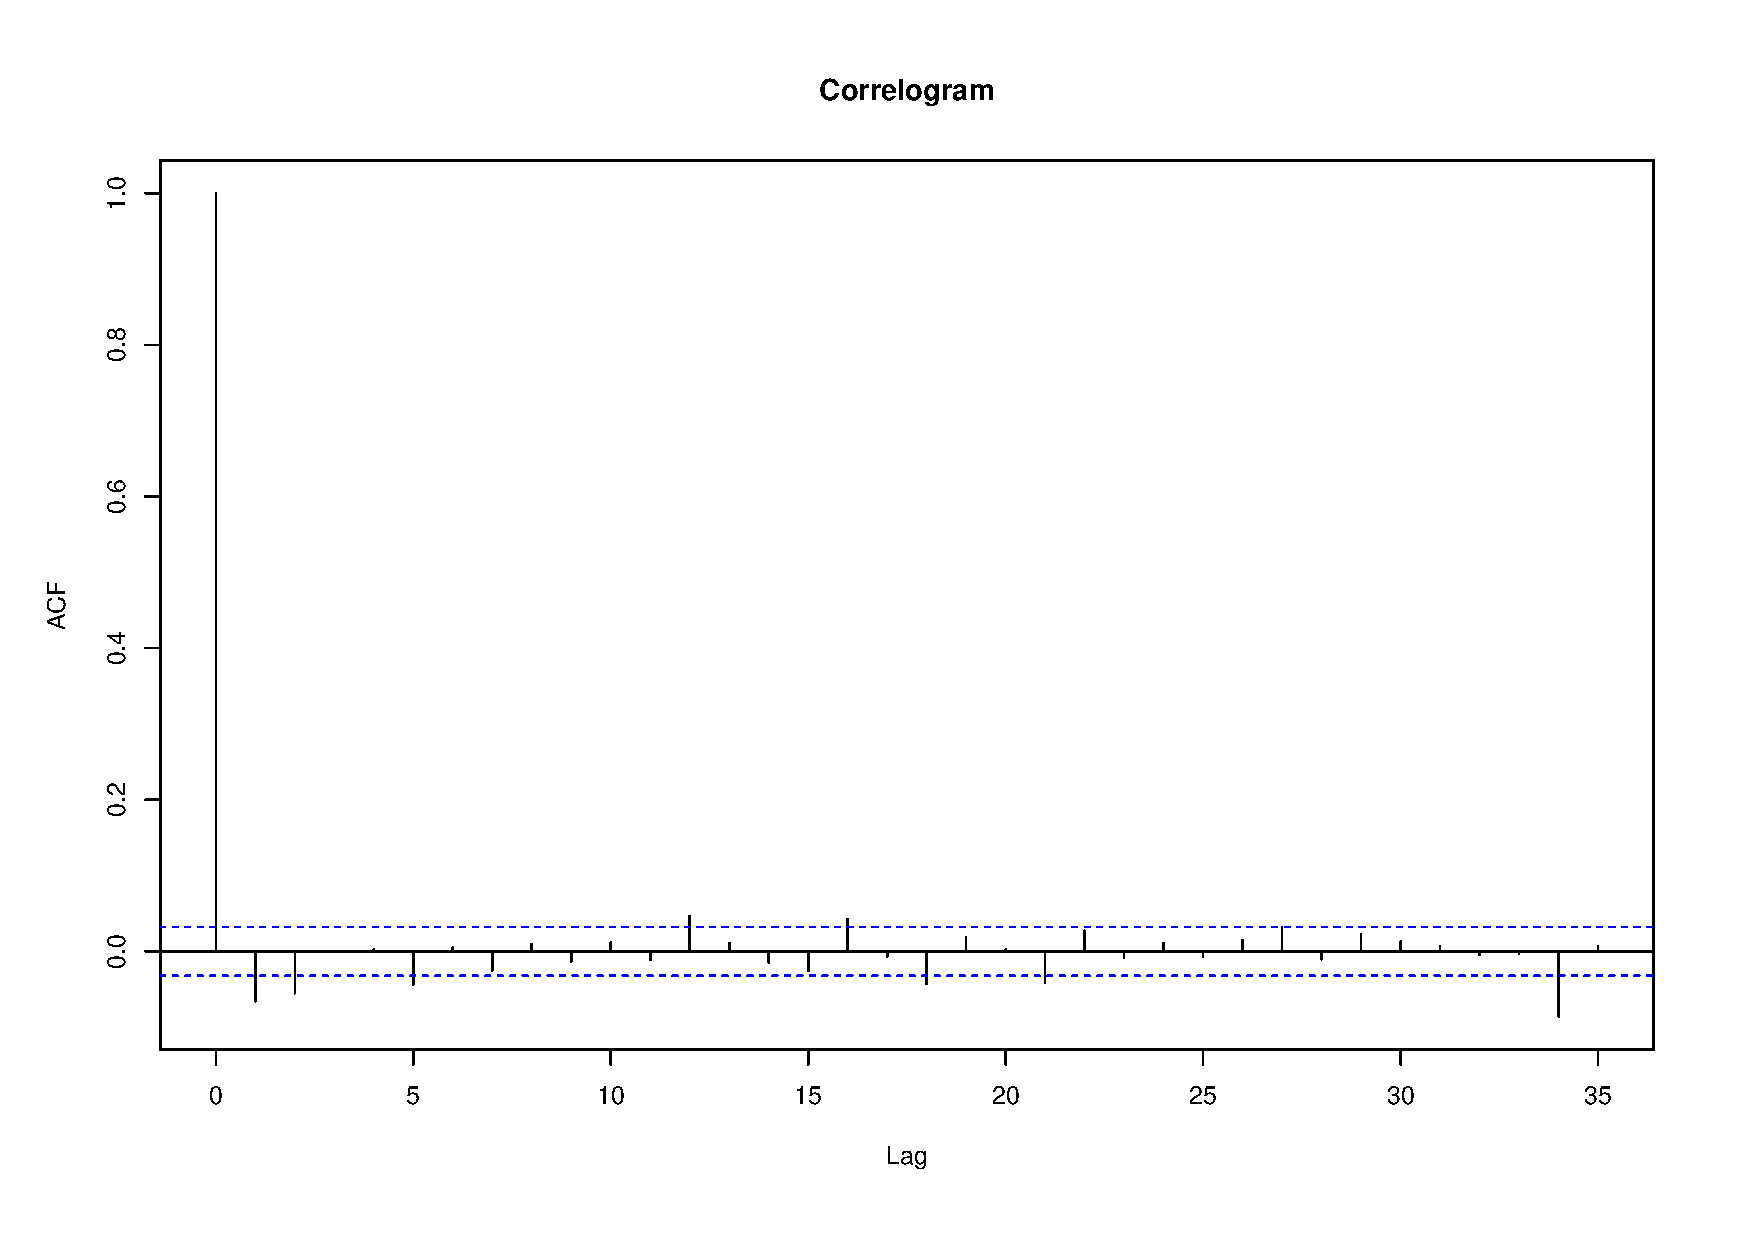
\includegraphics[scale=0.5]{plots/spy_returns_acf.pdf}
 % spy_returns_dist.pdf: 504x504 pixel, 72dpi, 17.78x17.78 cm, bb=0 0 504 504
 \caption{SPY returns ACF}
 \label{fig:returnacf}
\end{figure}

 \item[Returns distribution] The returns distribution has fat tails, i.e. the number of extreme events (either positive or negative) returns is larger than what is hypothesized by common data generation process (generally normal distribution assumption). In the markets, fat tails are an undesirable feature because of the additional risk they imply.
 In the figure \ref{fig:returndist} is shown the SPY returns distribution based on daily dates from the period 1st July 1998 to 4th April 2013. The distribution was compared against the normal distribution which clearly doesn't fit the data.  
 
 
 \begin{figure}[h]
 \centering
 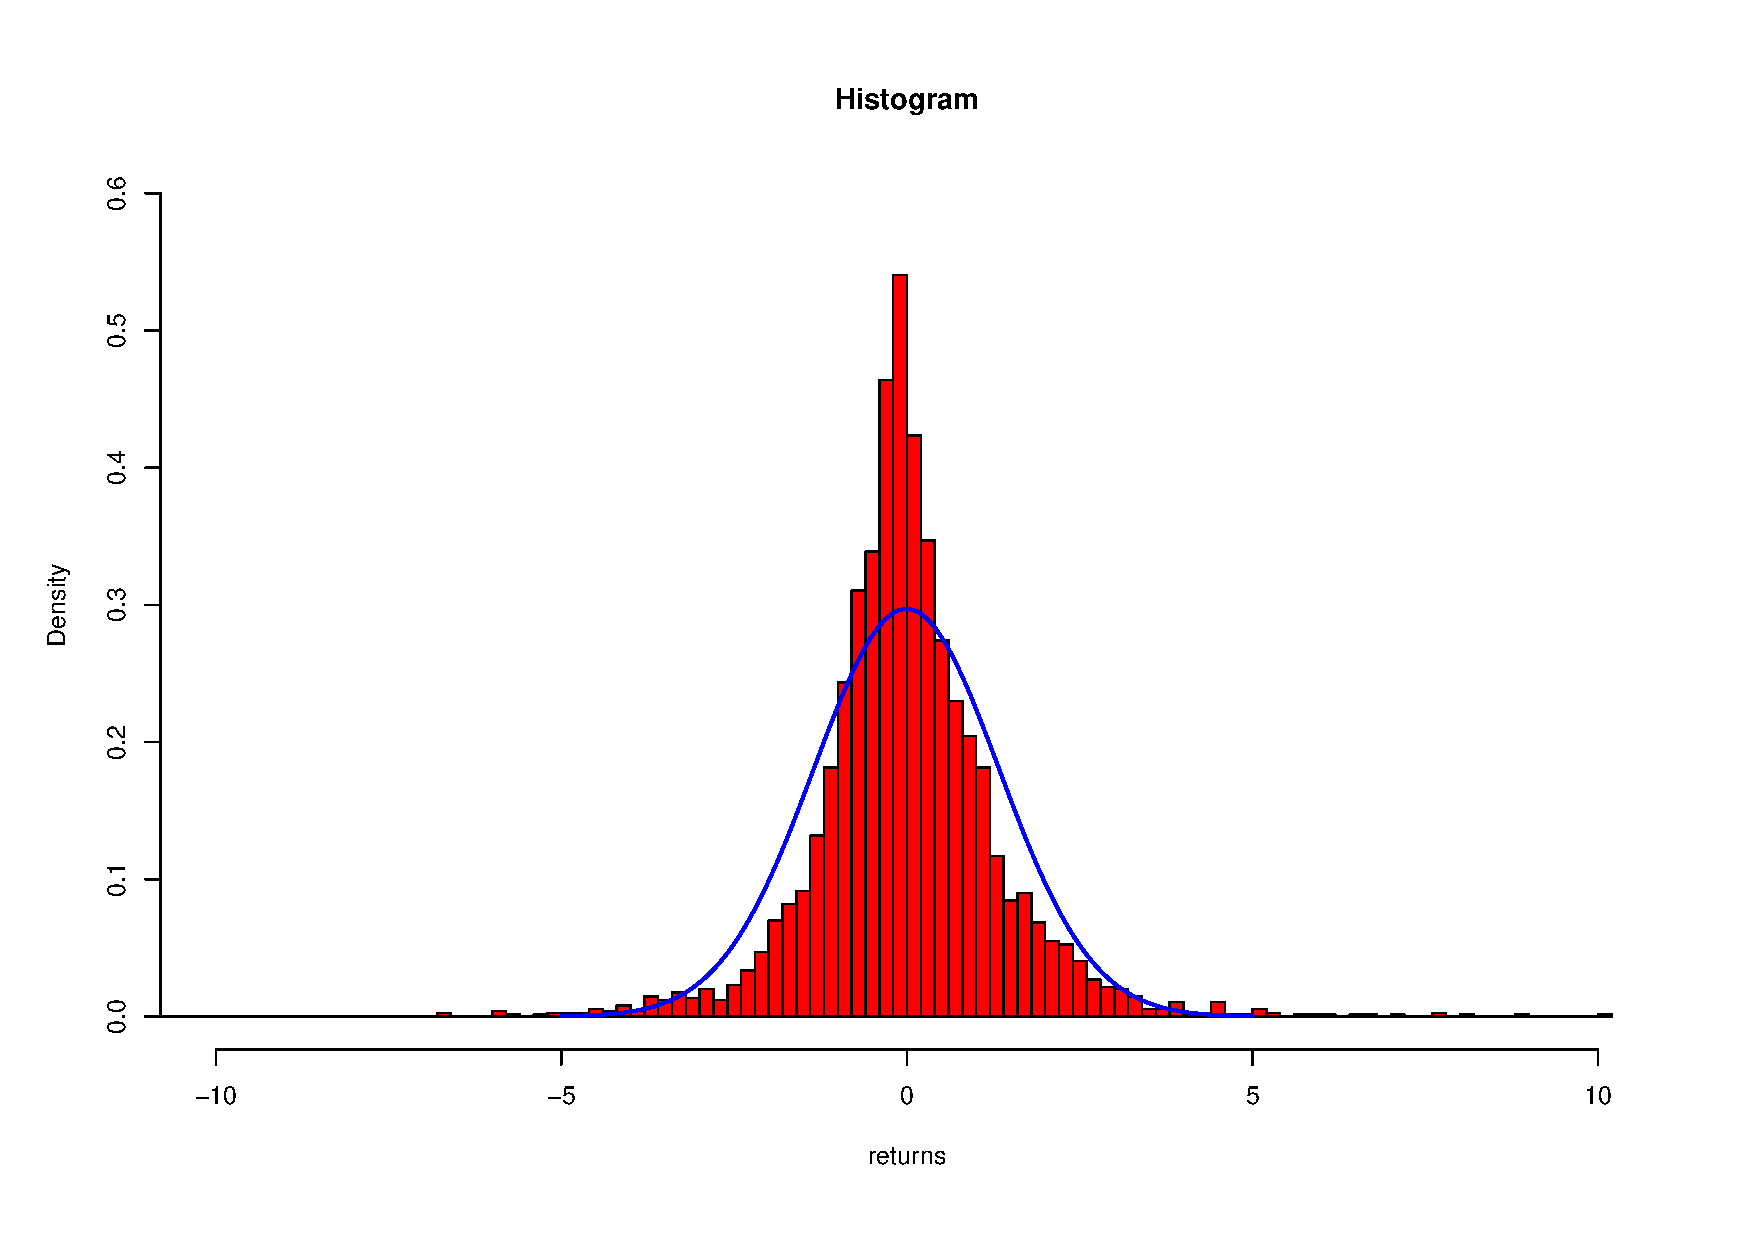
\includegraphics[scale=0.5]{plots/spy_returns_dist.pdf}
 % spy_returns_dist.pdf: 504x504 pixel, 72dpi, 17.78x17.78 cm, bb=0 0 504 504
 \caption{SPY returns distribution}
 \label{fig:returndist}
\end{figure}

 \item[Volume] refers to the level of trading activity in a market.
 \item[Calendar effects] days of week, weekend, holidays.
 \item[Intraday effects] time of the day.
 \item[Overnight effects]
\end{description}


%Autocorrelation
%Agregar gráficos de ACF de retornos y volatilities

\chapter{Implied volatility models}

\section{Black-Scholes formula}

In finance, an option is a derivative, that is, a contract which gives the owner the right, but not the obligation to buy or sell an underlying asset at a given price called strike price. An option can be executed at any time before an expiration date previously defined no matter what price the underlying asset has. 

The Black-Scholes formula~\cite{black1973}, developed in the early 1970's, Myron Scholes, Robert Merton and Fisher Black,  allows to determine an option value $V$ based on the underlying asset price $S(t)$ at a time $t$ and the following constant parameters: 

\begin{description}
\item [$\sigma$:] underlying asset price volatility which measures the standard deviation of the returns
\item [$\mu$:] underlying asset drift which is a measure of the average rate of growth of the stock
\item[$E$:] option strike or excersice price
\item[$T$:] option date of expiry
\item[$t$:] current time
\item[$r$:] risk-free interest rate
\end{description}

\subsection{Stock price model}

The Black-Scholes model assume that the underlying price $S$ follows a lognormal random walk:

\begin{equation}\label{eq:stockprice}
dS = \mu S dt + \sigma S dB
\end{equation}

\noindent where $B$ is a Brownian motion. This stochastic differential equation has two components: a deterministic term given by $\mu S dt$ and a random term given by $\sigma S dX$.

\subsection{Brownian motion}

A brownian motion $B$ (also called a Wiener process) is a stochastic process characterized by the three following properties:

\begin{description}
\item[Continuity:] $B(t)$ is a continuos function
\item[Normal increments:]  $B(t)-B(s)$ has a normal distribution with mean $0$ and variance $t-s$.
\item[Independence of increments:] for every choice of nonnegative real numbers $0 \leq s_1 <  t_1 \leq \cdots \leq s_n < t_n < \infty$, the increment random variables $W_{t_1} - W_{s_1}, \cdots, W_{t_n} - W_{s_n}$ are jointly independent.
\end{description}

\subsection{Stochastic differential equation}

An stochastic differential integral has the form:


\begin{equation}
W(T)=\int_0^T f(t)dB(t) \, .
\end{equation}

\noindent This equations is also expressed in an abbreviate form:

\begin{equation}
dW = f(t) dB \, .
\end{equation}

\noindent Therefore, the integral form of the stock price model shown in equation (\ref{eq:stockprice}) is:

\begin{equation}
S(T)=\int_0^T \mu S(t) dt + \int_0^T \sigma S(t) dB(t)
\end{equation}

\subsection{Ito's Lemma}

Ito's lemma is used to find the differential of a time dependent function of a stochastic process. In option pricing we need to find the option price $V(S(t))$ which depends on a stochastic stock price model $S(t)$. 
$V(S,t)$ is required to be  differentiable function of $S$ and once differentiable function of $t$.





%These are known or can be easily obtained from the market, excepting by volatility which must be estimated. However, rather than assuming a volatility a priori and computing option prices from it, the model can be used to estimate volatility at given prices, time to expiration and strike price. This obtained volatility is called the implied volatility of an option. Additionally, some models obtain implied volatility from futures (other derivative from prices). 


 

\chapter{Realized Volatility Models}

\section{GARCH}
test
\section{ARFIMA}
\section{Stochastic Volatility}
\chapter{Machine Learning Models}
\section{Batch learning}
\section{Online learning}


%\include{chap2}


%\appendix
%\chapter{Tables}

\begin{table}
\caption{Armadillos}
\label{arm:table}
\begin{center}
\begin{tabular}{||l|l||}\hline
Armadillos & are \\\hline
our	   & friends \\\hline
\end{tabular}
\end{center}
\end{table}

\clearpage
\newpage

%\chapter{Figures}

\vspace*{-3in}

\begin{figure}
\vspace{2.4in}
\caption{Armadillo slaying lawyer.}
\label{arm:fig1}
\end{figure}
\clearpage
\newpage

\begin{figure}
\vspace{2.4in}
\caption{Armadillo eradicating national debt.}
\label{arm:fig2}
\end{figure}
\clearpage
\newpage

%% This defines the bibliography file (main.bib) and the bibliography style.
%% If you want to create a bibliography file by hand, change the contents of
%% this file to a `thebibliography' environment.  For more information 
%% see section 4.3 of the LaTeX manual.
\begin{singlespace}
%\bibliography{main}
\bibliographystyle{plain}
\bibliography{reference}
\end{singlespace}

\end{document}

